\section{State of research}
\label{sec:state_of_research}
This chapter provides an overview of related researches in the field of software evolution analysis. The related work addresses how information of version control and issue tracking systems can be investigated by using specific analyzation methods.

%Populating a Release History Database from Version Control and Bug Tracking Systems:
\subsection{Release History Database}
The anlayzation method by Fischer et al. \cite{fischer2003populating} uses a release history database (RHDB) to research the software evolution of development projects. The RHDB is populated with version data of version control systems called modification reports (MR) and bug tracking data of bug repositories called problem reports (PR). Once the RHDB is populated, it is possible to execute simple queries to the structured data. Those queries produce specific views that enable an accurate reasoning of evolutionary aspects of software evolution \cite{fischer2003populating}.
Fischer et al. tested their approach on the large Open Source project Mozilla Firefox \cite{mozilla}. In this project, the analyzed version control data is managed with the CVS \cite{cvs} system, while the bug data is stored in the Bugzilla \cite{bugzilla} issue tracking system. \\

To populate the RHDB, Fisher et al. extracted the data of both systems and imported it into the database. This was implemented by different Shell and Perl scripts that process the data and inserted it into the RHDB. \\
For linking the MR and PRs the scripts used regular expressions to find ID-numbers which could link to the PRs. Ofcourse this data has lower quality since it is not clear whether the found numbers where the ids or other kind of information. Their matching is rated according to three difrent confidence values "h" for high, "m" for medium and "l" for low confidence. A quality improvment is achieved by checking the file names specified in the PR and the files commited or explained in the commit message. If this is the case the confidence value is changed from lower case to upper case. These rating values are stored as MR-PR relationships in the database.\\

The entity relationship (ER) model of the RHDB is shown in figure \ref{fig:rhdber} \cite{fischer2003populating}. There are according tables for data of the CVS version control system and the issue tracking system. For the CVS repository information, the important tables are \textbf{cvsitem}, \textbf{cvsitemlog} and \textbf{cvsauthor}. Therefore, the CVS artifact attributes are stored in the \textbf{cvsitem} table. Modification report data is stored in \textbf{cvsitemlog} and the author name of every CVS artifact is stored in the \textbf{cvsauthor} table. However, the bug report artifacts are stored in the \textbf{bugreport} table, whereas the description of a bug is stored in the \textbf{bugreportdesc} table. The connection between \textbf{cvsitemlog} and \textbf{bugreport} would be a n:n relation, hence it is resolved by a \textbf{cvsitemlogbugreport} table.\\

\begin{figure*}[t]
	\centering
	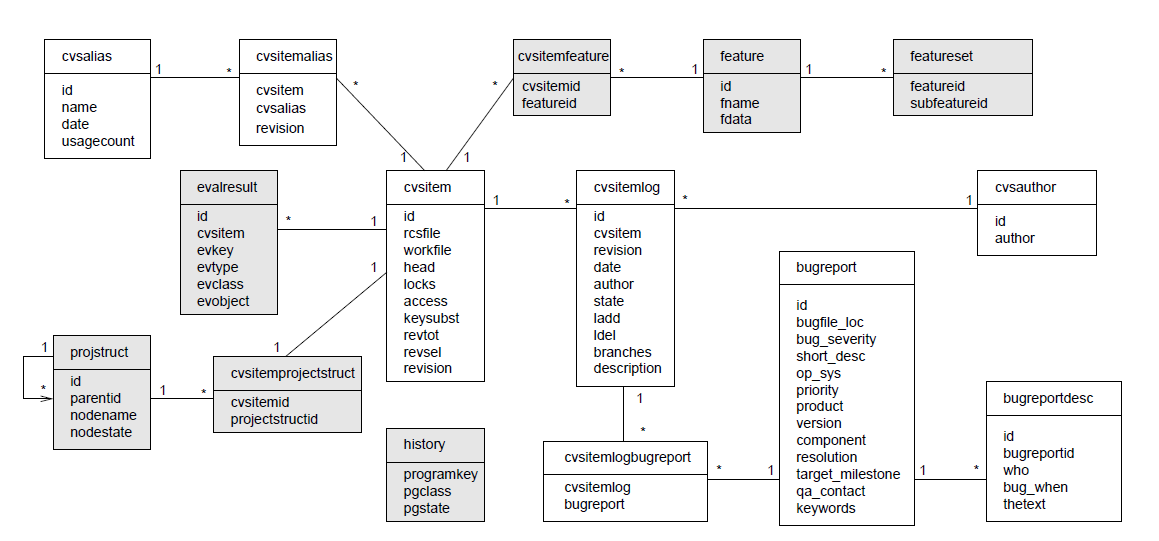
\includegraphics[width=0.8\textwidth]{images/rhdb_er}
	\caption{RHDB ER-Model \cite{fischer2003populating}}
	\label{fig:rhdber}
\end{figure*}

With this RHDB ER-Model it is possible to execute SQL-queries that can present a view on software evolution of the project. A sample query to list all bug reports for \textit{nsNSSDialogs.cpp}, presented by Fischer et al. is e.g. \cite{fischer2003populating}:

\begin{verbatim}
SELECT
	b.bugreport, r.bug_severity, r.short_desc
FROM
	cvsitem i, cvsitemlog l,
	cvsitemlogbugreport b, bugreport r
WHERE 	
	i.id = l.cvsitem
	AND l.id = b.cvsitemlog
	AND b.bugreport = r.id
	AND i.rcsfile REGEXP 'nsNSSDialogs.cpp';
	
\end{verbatim}

The application of the method on the Mozilla project stated that it was possible to link bug reports with version control data in an effective way \cite{fischer2003populating}. 

\subsection{Commit Message Standard}
Code developing should not start until a commit message standard has been established. Otherwise many programmer only writer commit messages since it has to be done, like shown in figure \ref{git_commit}. By unifying the commit messages, they can be read with more ease and automatically processed by an algorithm. \\

\begin{figure}[b]
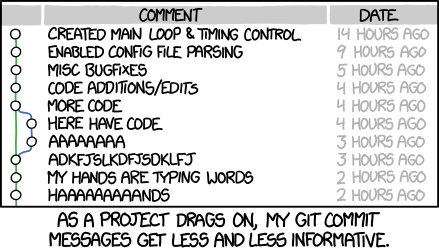
\includegraphics[width=0.5\textwidth]{images/git_commit.png}
\caption{Bad practice example}
\label{git_commit}
\end{figure}

A good commit message standard suggests that a report should consist of a \textit{task reference}, \textit{commit type} and a \textit{Description}. Always try to use imperative speech, for instance "Implement Class", not "Implemented Class" or "Implementing Class". 
\paragraph{Task reference}
By connecting tasks and commit messages developer can easily relate code to the issues. Also many bug tracker or task scheduler like redmine use the information to display the commit messages in the different task or issues.
\paragraph{Commit Type}
Commit types can be \textit{Fix}, \textit{Implement}, \textit{Refactor} or \textit{Update}. This gives the readers a quick overview of purpose of the modification.
\paragraph{Description}
Here, try to summarize the changes in about 50 characters. 
If necessary explain the causing problem or the feature being implemented in more detail in a new paragraph using about 72 characters. By using indents or bullet points the readability can be heavily improved. Bullet points are usually hyphons or asterisks follwed by a blank space and are separated by an empty line.
\\\\
Always try to address only one issue or task on each commit message. If inevitable separate the descriptions leaving a line blank.


%Wie hat sich die Wissenschaft bis jetzt entwickelt?
%Wer hat welche Voraussetzungen geschaffen?
%Welche vergleichbaren Ergebnisse gibt es bisher?
%Welche Fragen sind noch offen?
%Warum reicht das bisher Getane noch nicht?
%Soll eine bestimmte These widerlegt oder bestätigt werden?
%Welche sind die wichtigen Veröffentlichungen? Was sagen sie zum Thema?